\documentclass[tikz, border=20pt]{standalone}
\usepackage{amsmath, amssymb}
\usetikzlibrary{calc, positioning, arrows.meta, backgrounds, fit}

% Move all styles here to prevent the optional argument parsing crash
\tikzset{
	font=\sffamily,
	% Panel and Title styles
	panel/.style={draw=darkgray!50, thick, rounded corners=12pt, fill=white},
	mainTitle/.style={font=\Huge\bfseries, text=darkgray, align=center},
	subTitle/.style={font=\Large\bfseries, text=darkgray, align=center},
	% Geometric Pentagon dot styles
	pdot1/.style={circle, fill=darkgray, draw=white, thick, inner sep=2.5pt},
	pdot2/.style={circle, fill=cyan!80!black, draw=white, thick, inner sep=2.5pt},
	pdot3/.style={circle, fill=magenta!80!black, draw=white, thick, inner sep=2.5pt},
	% Ferrers diagram dot styles
	fdot/.style={circle, fill=gray!80, inner sep=3pt},
	base/.style={circle, fill=blue!60, inner sep=3pt},
	slope/.style={circle, fill=red!60, inner sep=3pt},
	intersect/.style={circle, fill=purple!80, draw=black, thick, inner sep=3pt},
	% Arrow styles
	mapArrow/.style={->, >=Stealth, line width=2pt, color=darkgray, dashed}
}

\begin{document}
	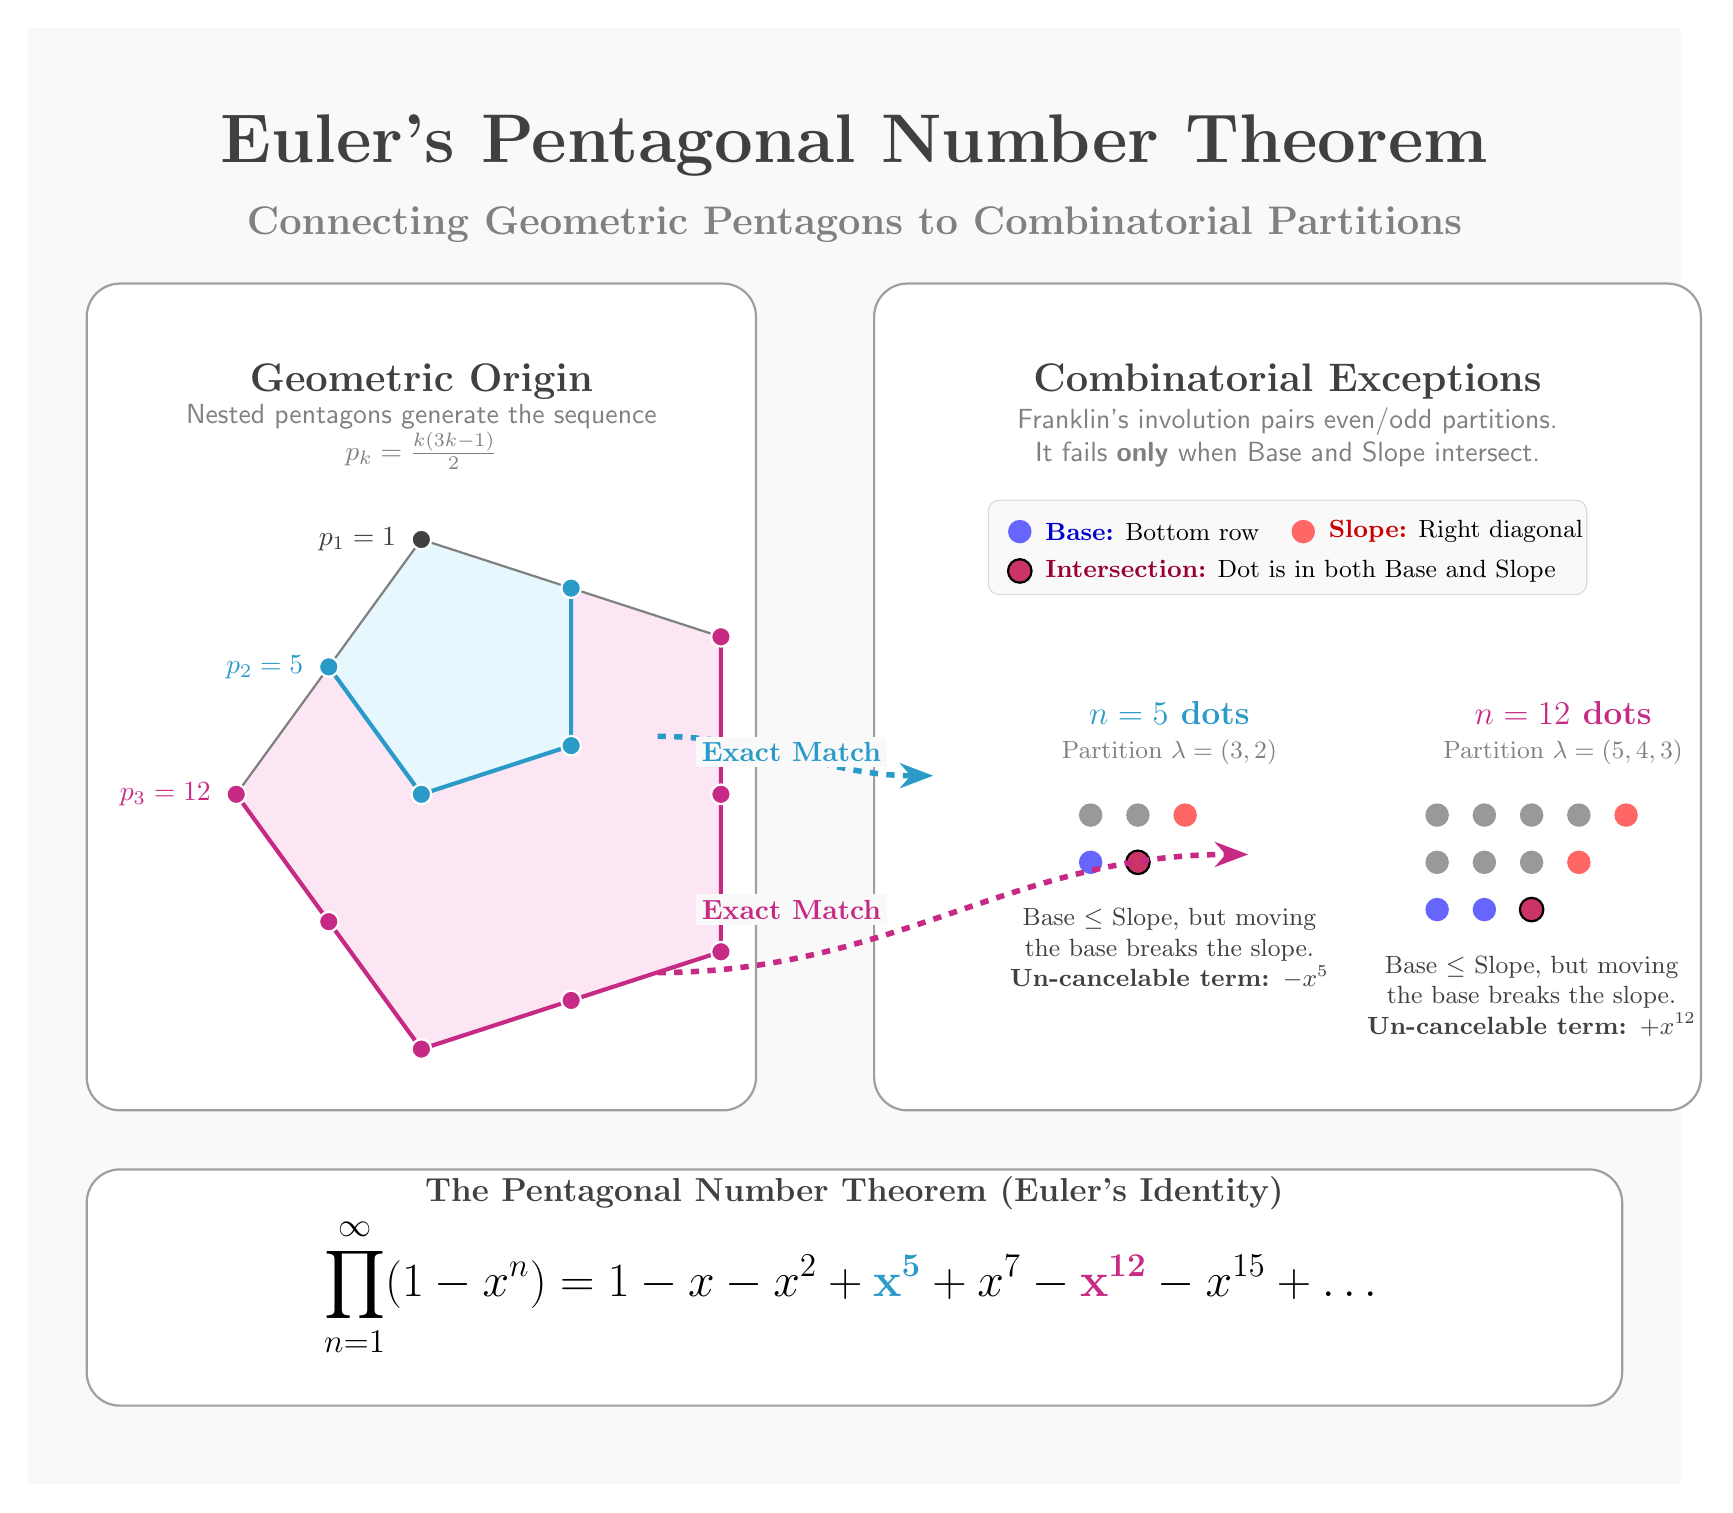
\begin{tikzpicture}
		
		% ==============================================================================
		% BACKGROUND
		% ==============================================================================
		\fill[gray!5] (-9, 8) rectangle (12, -10.5);
		
		% ==============================================================================
		% HEADER
		% ==============================================================================
		\node[mainTitle] at (1.5, 6.5) {Euler's Pentagonal Number Theorem};
		\node[subTitle, text=gray] at (1.5, 5.5) {Connecting Geometric Pentagons to Combinatorial Partitions};
		
		% ==============================================================================
		% LEFT PANEL: THE GEOMETRIC PENTAGONS
		% ==============================================================================
		\node[panel, minimum width=8.5cm, minimum height=10.5cm] (GeomPanel) at (-4, -0.5) {};
		\node[subTitle] at (-4, 3.5) {Geometric Origin};
		\node[align=center, text=gray] at (-4, 2.8) {Nested pentagons generate the sequence\\$p_k = \frac{k(3k-1)}{2}$};
		
		\begin{scope}[shift={(-4, 1.5)}]
			% Define Coordinates using turtle graphics for exact regular pentagon edges
			\coordinate (V0) at (0,0);
			
			% k=2 Pentagon (d=2)
			\path (V0) ++(234:2) coordinate (V1) ++(306:2) coordinate (V2) ++(18:2) coordinate (V3) ++(90:2) coordinate (V4);
			
			% k=3 Pentagon (d=4)
			\path (V0) ++(234:4) coordinate (W1) ++(306:4) coordinate (W2) ++(18:4) coordinate (W3) ++(90:4) coordinate (W4);
			
			% Midpoints for k=3
			\coordinate (M1) at ($(W1)!0.5!(W2)$);
			\coordinate (M2) at ($(W2)!0.5!(W3)$);
			\coordinate (M3) at ($(W3)!0.5!(W4)$);
			
			% Draw Areas
			\fill[magenta!10, rounded corners=4pt] (V0) -- (W1) -- (W2) -- (W3) -- (W4) -- cycle;
			\fill[cyan!10, rounded corners=4pt] (V0) -- (V1) -- (V2) -- (V3) -- (V4) -- cycle;
			
			% Draw Lines
			\draw[thick, gray] (V0) -- (W1);
			\draw[thick, gray] (V0) -- (W4);
			\draw[line width=1.5pt, cyan!80!black] (V1) -- (V2) -- (V3) -- (V4);
			\draw[line width=1.5pt, magenta!80!black] (W1) -- (W2) -- (W3) -- (W4);
			
			% Draw Dots (Layered from largest to smallest)
			\foreach \p in {W1, M1, W2, M2, W3, M3, W4} \node[pdot3] at (\p) {};
			\foreach \p in {V1, V2, V3, V4} \node[pdot2] at (\p) {};
			\node[pdot1] at (V0) {};
			
			% Labels
			\node[font=\bfseries, text=darkgray, left] at ($(V0)+(-0.2, 0)$) {$p_1 = 1$};
			\node[font=\bfseries, text=cyan!80!black, left] at ($(V1)+(-0.2, 0)$) {$p_2 = 5$};
			\node[font=\bfseries, text=magenta!80!black, left] at ($(W1)+(-0.2, 0)$) {$p_3 = 12$};
		\end{scope}
		
		% ==============================================================================
		% RIGHT PANEL: FRANKLIN's COMBINATORIAL EXCEPTIONS
		% ==============================================================================
		\node[panel, minimum width=10.5cm, minimum height=10.5cm] (CombPanel) at (7, -0.5) {};
		\node[subTitle] at (7, 3.5) {Combinatorial Exceptions};
		\node[align=center, text=gray] at (7, 2.8) {Franklin's involution pairs even/odd partitions.\\It fails \textbf{only} when Base and Slope intersect.};
		
		% Legend for Ferrers Diagram (Safely coded to avoid nested tikzpictures)
		\begin{scope}[shift={(3.2, 0.8)}]
			\draw[draw=gray!30, rounded corners, fill=gray!5] (0,0) rectangle (7.6, 1.2);
			\node[base] at (0.4, 0.8) {}; \node[right, font=\small] at (0.6, 0.8) {\textcolor{blue!80!black}{\textbf{Base:}} Bottom row};
			\node[slope] at (4.0, 0.8) {}; \node[right, font=\small] at (4.2, 0.8) {\textcolor{red!80!black}{\textbf{Slope:}} Right diagonal};
			\node[intersect] at (0.4, 0.3) {}; \node[right, font=\small] at (0.6, 0.3) {\textcolor{purple!80!black}{\textbf{Intersection:}} Dot is in both Base and Slope};
		\end{scope}
		
		% Exception 1: n=5
		\begin{scope}[shift={(4.5, -1.5)}]
			\node[font=\large\bfseries, text=cyan!80!black] at (1, 0.8) {$n=5$ dots};
			\node[font=\small, text=gray] at (1, 0.3) {Partition $\lambda = (3, 2)$};
			
			% Row 1
			\node[fdot] at (0, -0.5) {}; \node[fdot] at (0.6, -0.5) {}; \node[slope] at (1.2, -0.5) {};
			% Row 2
			\node[base] at (0, -1.1) {}; \node[intersect] at (0.6, -1.1) {};
			
			\node[align=center, font=\small, text=darkgray] at (1, -2.2) {
				Base $\le$ Slope, but moving\\the base breaks the slope.\\\textbf{Un-cancelable term: $-x^5$}
			};
		\end{scope}
		
		% Exception 2: n=12
		\begin{scope}[shift={(9.5, -1.5)}]
			\node[font=\large\bfseries, text=magenta!80!black] at (1, 0.8) {$n=12$ dots};
			\node[font=\small, text=gray] at (1, 0.3) {Partition $\lambda = (5, 4, 3)$};
			
			% Row 1
			\node[fdot] at (-0.6, -0.5) {}; \node[fdot] at (0, -0.5) {}; \node[fdot] at (0.6, -0.5) {}; \node[fdot] at (1.2, -0.5) {}; \node[slope] at (1.8, -0.5) {};
			% Row 2
			\node[fdot] at (-0.6, -1.1) {}; \node[fdot] at (0, -1.1) {}; \node[fdot] at (0.6, -1.1) {}; \node[slope] at (1.2, -1.1) {};
			% Row 3
			\node[base] at (-0.6, -1.7) {}; \node[base] at (0, -1.7) {}; \node[intersect] at (0.6, -1.7) {};
			
			\node[align=center, font=\small, text=darkgray] at (0.6, -2.8) {
				Base $\le$ Slope, but moving\\the base breaks the slope.\\\textbf{Un-cancelable term: $+x^{12}$}
			};
		\end{scope}
		
		% ==============================================================================
		% CONNECTING ARROWS (Mapping Geometry to Combinatorics)
		% ==============================================================================
		% To n=5
		\draw[mapArrow, draw=cyan!80!black] (-1, -1) to[out=0, in=180] (2.5, -1.5);
		\node[font=\bfseries, text=cyan!80!black, fill=gray!5, inner sep=2pt] at (0.7, -1.2) {Exact Match};
		
		% To n=12
		\draw[mapArrow, draw=magenta!80!black] (-1, -4) to[out=0, in=180] (6.5, -2.5);
		\node[font=\bfseries, text=magenta!80!black, fill=gray!5, inner sep=2pt] at (0.7, -3.2) {Exact Match};
		
		% ==============================================================================
		% BOTTOM PANEL: THE EQUATION
		% ==============================================================================
		\node[panel, minimum width=19.5cm, minimum height=3cm] (EqPanel) at (1.5, -8) {};
		
		\node[font=\LARGE, text=black] at (1.5, -8) {
			$\displaystyle \prod_{n=1}^\infty (1-x^n) = 1 - x - x^2 + \textcolor{cyan!80!black}{\mathbf{x^5}} + x^7 - \textcolor{magenta!80!black}{\mathbf{x^{12}}} - x^{15} + \dots$
		};
		
		\node[font=\large\bfseries, text=darkgray] at (1.5, -6.8) {The Pentagonal Number Theorem (Euler's Identity)};
		
	\end{tikzpicture}
\end{document}